\documentclass[11pt,letterpaper]{article}
\usepackage[margin=1in]{geometry}
\usepackage{graphicx}
\usepackage{hyperref}
\usepackage{listings}
\pagestyle{headings}
\usepackage{epstopdf}

\begin{document}

\title{PHY 410 \\ Homework Assignment 2}
\author{Han Wen \\ \tiny Person No. 50096432}
\date{\today}

\maketitle

\begin{abstract}
The goal of this assignment was to use numerical method to analyse some earth quake data and those regarding global warming as well.
\end{abstract}

\tableofcontents

\newpage
\section{Problem 1}

\subsection{Description}
Download the NEIC Global data set of earthquakes with magnitudes greater than 1.0 and use a quake.cpp code to fit the Gutenberg Richter Law. The raw data do not provide a reasonable fit. Explain why and fix the code to obtain a more reliable estimate of the slope constant  . Check your answer with values given in the references from class\cite{The Physics of Earthquakes}




\subsection{Numerical Analysis}
The “Richter scale” was developed by Richter in the 1930’s, relates the local magnitude scale $M_L$ defined by the amount of amplitude variation on a seismograph \cite{Seismographs and Seismograms}. In the 1970's, the moment magnitude scale was introduced given by $M_0=muSD$. Additionally, the Gutenberg-Richter Model gives the relationship of the frequency(N) of the earthquakes and the corresponding magnitude of them. The frequency defined as the number of events with magnitude greater or equal to M, namely the Empirical model:
$logN=a-bM$
Therefore we are going to do a linear fits with $logN$ and $M$ and obtain the slope.

\subsection{Results}

Noticing the original code didn't choose the data homogeneously and apparently those with smaller magnitude and bigger magnitude has different slope, considering the bigger the earthquake is the more concern we have about it, we are going to only use those have magnitudes bigger or equal to 4 and choose points homogeneously in that interval, then plot and calculate the slope. Here is the plot ~\ref{figure1} 
, the slope will be $b=-0.814\pm0.076$, compared to the value about $-1$ in the article \cite{The Physics of Earthquakes}, it's a little smaller and considering we only use the data from last 3 years and in specifically California area, the discrepancy is accepted.
 
\begin{figure}
\begin{center}
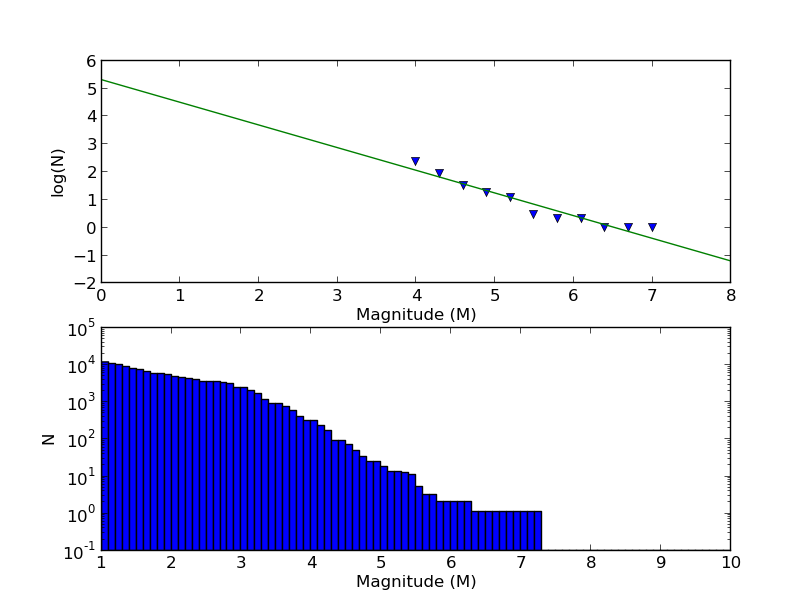
\includegraphics[width=0.6\linewidth,angle=0]{quake.png}
\caption{The earthquake using CA data.}
\label{figure1}
\end{center}
\end{figure}




\newpage

\section{Problem 2}

\subsection{Description}

Download the NOAA Mauna Loa CO  data set (ALSO included in the lecture 6 example code, if the link is not working) and modify the co2.cpp or co2.py code to generate graphs using other columns in the data. Does the average rate of increase depend on which colums are used in a straight line fit? Explore linear models with 3 terms to decide whether the linear rate of increase is accelerating or decelerating. If the current rate of increase continues indefinitely, when will the concentration become toxic (50,000 ppm)?

\subsection{Result}

Using the average value, we have the slope $b=1.474\pm0.009$, with the plot ~\ref{figure2} 

Using the interpolated value, we have the slope $b=1.470\pm0.009$, with the plot ~\ref{figure3} 

Using the trend value, we have the slope $b=1.472\pm0.007$, with the plot ~\ref{figure4}. 

So we can see the average rate of increase basically remains the same. 
With the data of average value, I did a linear fits using three different interval of data, namely the first part 1958-1976 middle part 1976-1995 and last part 1995-2014, and the average rates of increase are  0.95 1.53 1.95; for average one it's 0.95,1.51,1.94; for trend one it's 0.95,1.52,1.95. So the rate of increase is increasing. With this trend, after 25411 years it will become toxic. 


\begin{figure}
\begin{center}
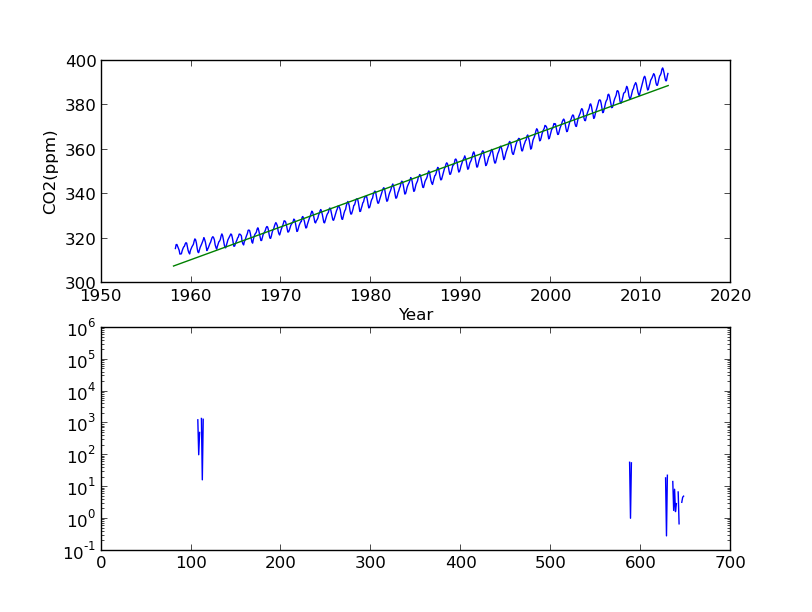
\includegraphics[width=0.6\linewidth,angle=0]{q2ave.png}
\caption{the CO2 with average.}
\label{figure2}
\end{center}
\end{figure}


\begin{figure}
\begin{center}
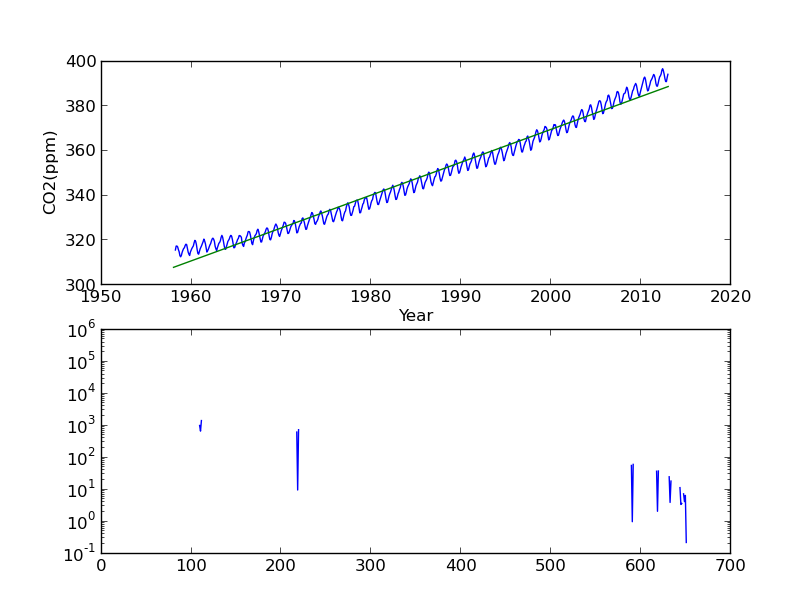
\includegraphics[width=0.6\linewidth,angle=0]{q2inter.png}
\caption{the CO2 with interpolated.}
\label{figure3}
\end{center}
\end{figure}

\begin{figure}
\begin{center}
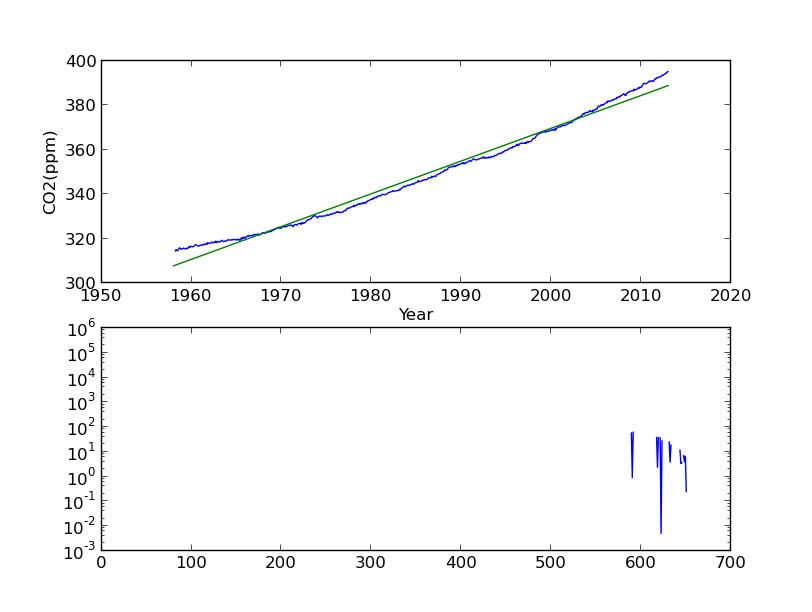
\includegraphics[width=0.6\linewidth,angle=0]{q2tre.png}
\caption{the CO2 with trend.}
\label{figure4}
\end{center}
\end{figure}






\newpage

\section{Problem 3}
\subsection{Description}
Earthquake Problem: Find a different event data set (e.g. from the Southern California Earthquake Center http://www.scec.org/resources/data/, or any other source you can find on the Web), perform a linear fit and compare your results with the NEIC global set.

Global Warming Problem: Download a NASA Global Temperature Anomaly data set for a similar time period as the NOAA Mauna Loa data and analyze the trend. Can you conclude from your analysis that the two sets are correlated in any way?
\subsection{Numerical analysis} 
For earthquake, I got the data from National Climatic Data Center \cite{NCDC}, from year 1932 to 1999

For CO2, I got data from Earth System Research Laboratory \cite{ESRL} from 1969 to 2005

\subsection{Result}

For earthquake: the calculated slope is $b=-0.921\pm0.018$, with the plot ~\ref{figure5}, we can see it's more close to the accepted value in that article.

For CO2: With those data the calculated slope is $b=1.655\pm0.011$, with the plot ~\ref{figure6}, the number is bigger than the above ones but not too much, probably because the sample is smaller and in the earlier time this data is incomplete. However, the trend is very similar, the general trend is increasing but will vibrate locally.   



\begin{figure}
\begin{center}
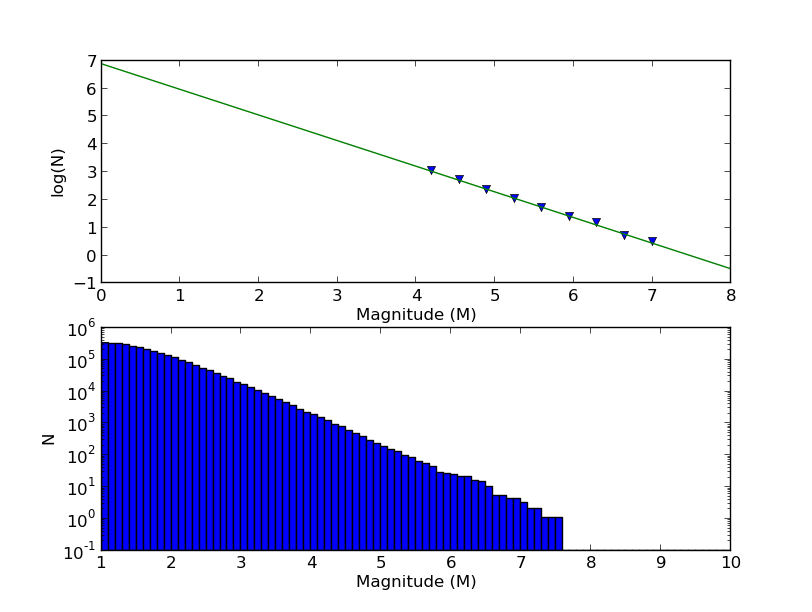
\includegraphics[width=0.6\linewidth,angle=0]{quake3.png}
\caption{Earthquake 1932-1999}
\label{figure5}
\end{center}
\end{figure}

\begin{figure}
\begin{center}
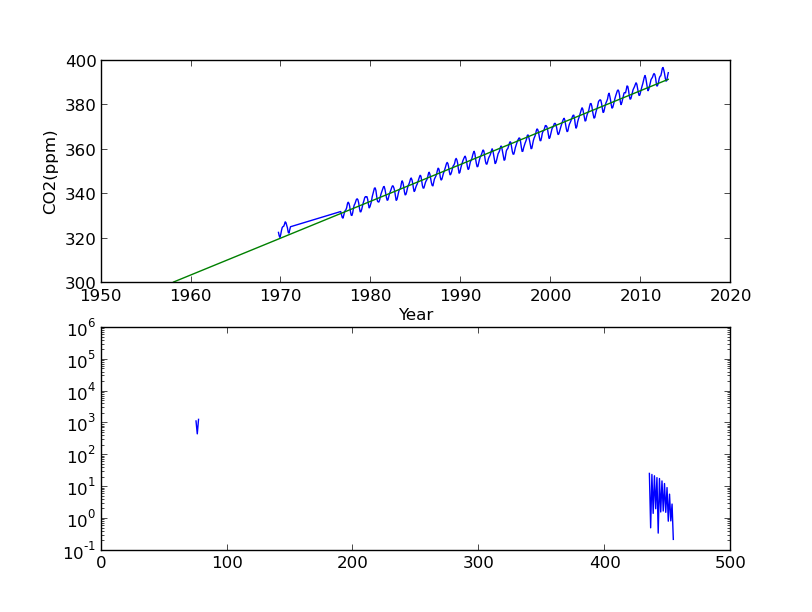
\includegraphics[width=0.6\linewidth,angle=0]{q3.png}
\caption{CO2 1969-2005}
\label{figure6}
\end{center}
\end{figure}




\newpage
\section*{Acknowledgements}

I discussed this assignment with my classmates and used material from the
cited references, but this writeup is my own.

\begin{thebibliography}{9}

\bibitem{The Physics of Earthquakes}
H. Kanamori and E.E. Brodsky, The Physics of Earthquakes, Physics Today 54, 34-40 (2001)\url{http://scitation.aip.org/content/aip/magazine/physicstoday/article/54/6/10.1063/1.1387590}

\bibitem{coursepage}
PHY 410-505 Webpage, \url{http://www.physics.buffalo.edu/phy410-505}.

\bibitem{Seismographs and Seismograms}
a brief introduction to seismographs and seismograms,\url{http://www.colorado.edu/physics/phys2900/homepages/Marianne.Hogan/graphs.html}.

\bibitem{NCDC}
National Climatic Data Center data base \url{ftp://ftp.ncdc.noaa.gov/pub/data/anomalies/anomalies/usingGHCNMv2/}

\bibitem{ESRL}
Mauna Loa, Hawaii, United States(MLO), monthly averages
\url{http://www.esrl.noaa.gov/gmd/dv/data/index.php?site=mlo&category=Greenhouse%2BGases&parameter_name=Carbon%2BDioxide}

\end{thebibliography}

\newpage
\appendix
\section{Appendix}

\subsection{python code}

The following python code was used to obtain the results in this report:

\lstinputlisting[language=python]{co2.py}

\lstinputlisting[language=python]{quake.py}

\end{document}
